p\section{Introduction}
Artist identification is traditionally performed by \textit{art historians} and \textit{curators} who have expertise and familiarity with different artists and styles of art. This is a complex and interesting problem for computers because identifying an artist does not just require object or face detection; artists can paint a wide variety of objects and scenes. Additionally, many artists from the same time period will have similar styles, and some such as \textbf{Pablo Picasso} (see figure \ref{fig:picasso}) have painted in multiple styles and changed their style over time.

\begin{figure}[H]
	\centering
	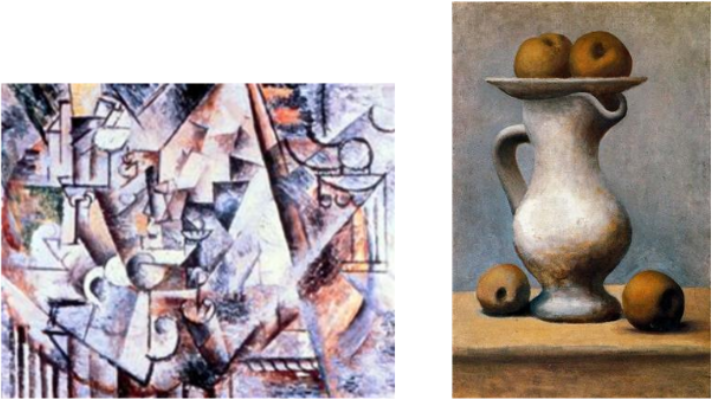
\includegraphics[width=0.4\textwidth]{img/picasso.png}
	\caption{Both of these paintings were created by Pablo Picasso, but they have vastly different styles and content since they correspond to two different periods.}
	\label{fig:picasso}
\end{figure}

\noindent The aim of this project is to use Convolutional Neural Networks for the identification of an artist given a painting. In particular, the CNN networks will be modeled using multiple techniques: from scratch; via pretrained network; networks based on comparison with baseline input and using an ensemble network made of by the best classifiers found.


\subsection{State of the Art}
As mentioned, artist identification has primarily been tackled by humans. An example of that is the Artsy's Art Genome Project \footnote{https://www.artsy.net/categories}, which is led by experts who manually classify art. This strategy is not very scalable even if it is highly precise in the classification (the site is a marketplace of fine-arts for collects, you can find Pisarro, Bansky and other famous artists).

Most prior attempts to apply machine learning to this problem have been feature-based, aiming to identify what qualities most effectively distinguish artists and styles. Many generic image features have been used, including scale-invariant feature transforms (SIFT), histograms of oriented gradients (HOG), and more, but with the focus on \textit{discriminating different style} in Fine-Art Painting\footnote{T. E. Lombardi. The classification of style in fine-art paint-
ing. ETD Collection for Pace University, 2005}.

The first time the problem of artist identification was really tackled was with J. Jou and S. Agrawal\footnote{J. Jou and S. Agrawal. Artist identification for renaissance paintings.} in 2011, they applied several multi-class classification techniques like Naïve Bayes, Linear Discriminant Analysis, Logistic Regression, K-Means and SVMs and achieve a maximum classification accuracy of 65\% for an unknown painting across 5 artists. 
Later on, the problem of identifying artists was retackled by the \textit{Rijksmuseum Challenge}\footnote{T. Mensink and J. van Gemert. The rijksmuseum challenge: Museum-centered visual recognition. 2014}. The objective of the challenge was to predict the artist, type, material and creation year (each of them was a different challenge) of the 112,039 photographic \footnote{The dataset contains 6,629 artists in total, with high variation in the number of pieces per artist. For example, Rembrandt has 1,384 pieces, and Vermeer has only 4. There are 350 artists with more than 50 pieces, 180 artists have around 100, and 90 artists have 200 pieces.} (containing different viewpoints of an artwork, and different types of them: sculptures, paintings, saucers, etc.) reproductions of the artworks exhibited in the Rijksmuseum in Amsterdam (the Netherlands). For the artist classification challenge, the paper said they read a test accuracy of about 60\%. The year later, Saleh and Elgammal's paper\footnote{B. Saleh and A. M. Elgammal. Large-scale classification of fine-art paintings: Learning the right metric on the right
feature. CoRR, abs/1505.00855, 2015} was the first attempt to identify artists with a large and varied dataset, but still using generic features. The collection they used has images of 81,449 fine-art paintings from 1,119 artists ranging from fifteen centuries to contemporary artists, reaching an accuracy of 59\%\footnote{In the paper they tried to use also CNN, but reaching only an accuracy of 33.62\%}.


More recent attempts are related to the \textit{Painter by Numbers}, a \textbf{Playground Prediction Competition} by \textit{Kaggle}\footnote{https://www.kaggle.com/c/painter-by-numbers/data}. This competition used a pairwise comparison scheme: participants had to create an algorithm which needs to examine two images and predict whether the two images are by the same artist or not. Thus, it is not our same objective, however it can be consider the first application of Deep Learning to the problem. The real deal was taken by Nitin Viswanathan\footnote{Nitin Viswanathan, Artist Identification with Convolutional Neural Networks} in 2017.
Viswanathan, using the same dataset of the mentioned \textit{Kaggle Challenge}, proposed the use of ResNet with transfer learning (he first held the weights of the base ResNet constant and updated only the fully-connected layer for a few epochs). This trained network reached a train accuracy of 0.973 and a test accuracy of 0.898.



\subsection{Dataset}
Unfortunately, the dataset provided by the \textit{Kaggle Challange} is too huge to be used in Colab, in fact it is about 60GB unbearable on the free version of Colab, which provides only about 30GB of disk. Stated that, we decided to use a different dataset\footnote{https://www.kaggle.com/ikarus777/best-artworks-of-all-time} with only 2GB of data and about 8k unique images.

\noindent The data downloaded from Kaggle has the following directories and csv file:
\dirtree{%
.1 /.
.2 images.
.3 images.
.4 Albrecht\_Durer.
.4 Alfred\_Sisley.
.4 Amedeo\_Modigliani.
.4 Andrei\_Rublev.
.4 Andy\_Warhol.
.4 Camille\_Pissarro.
.4 Caravaggio.
.4 Claude\_Monet.
.4 Diego\_Rivera.
.4 Diego\_Velazquez.
.4 Edgar\_Degas.
.4 Edouard\_Manet.
.4 Edvard\_Munch.
.4 \textit{an many others (total of 50 different artists)}.
.2 resized.
.2 {artists.csv}.
}

\noindent The \textit{resized} directory is not useful for our studies, hence we deleted it to save space on the disk. On the other hand, we first use the \textit{csv} file to select only the artists with at least 200 pieces, this operation was done to reduce the number of classes to a number per which the ratio between the number of artists and images was reasonable for learning. Even done that, the dataset was still unbalanced, e.g. Van Gogh's paintings are 877 against the 239 of Chagall's, thus we consider to compute \textbf{class weights} in order to use them in the \textit{fit function}:

$
	\text{class\_weights} = \frac{\text{Total number of paintings considered}}{\text{Number of artists considered}\cdot \text{Number of paintings per author}}
$

\noindent Then, we modified the structure of the \textit{images/images} directory in order to create two directories, \textbf{train} and \textbf{test}, containing 90\% and 10\% of the images from each different artist's directory respectively (considering only the artists with at least 200 paintings). The newly created directories have the same structured of \textit{images/images}. This was done in \textit{python} in this way:

\begin{python}
import os
import numpy as np
import shutil

rootdir= '/content/images/images' #path of the original folder
classes = os.listdir(rootdir)

for i, c in enumerate(classes, start=1):
  if c not in artists_top_name.tolist():
    shutil.rmtree(rootdir + '/' + c)
    continue
  if not os.path.exists(rootdir + '/train/' + c):
    os.makedirs(rootdir + '/train/' + c)
  if not os.path.exists(rootdir + '/test/' + c):  
    os.makedirs(rootdir + '/test/' + c)

  source = os.path.join(rootdir, c)
  allFileNames = os.listdir(source)

  np.random.shuffle(allFileNames)

  test_ratio = 0.10
  train_FileNames, test_FileNames = np.split(np.array(allFileNames),
                                                        [int(len(allFileNames)* (1 - test_ratio))])

  train_FileNames = [source+'/'+ name for name in train_FileNames.tolist()]
  test_FileNames = [source+'/' + name for name in test_FileNames.tolist()]

  for name in train_FileNames:
    shutil.copy(name, rootdir +'/train/' + c)

  for name in test_FileNames:
    shutil.copy(name, rootdir +'/test/' + c)
\end{python}

After that we created the train/validation/test-sets using the \textit{image\_dataset\_from\_directory} function provided by \textbf{Keras} in the following way:

\begin{python}
import tensorflow as tf

training_images = tf.keras.preprocessing.image_dataset_from_directory(
    TRAIN_DIR, labels='inferred', label_mode='categorical',
    class_names=None, color_mode='rgb', batch_size=BATCH_SIZE, 
    image_size=(IMAGE_HEIGHT,  IMAGE_WIDTH), shuffle=True, seed=RANDOM_SEED, 
    validation_split=VALIDATION_SPLIT, subset='training',
    interpolation='bilinear', follow_links=False
)

val_images = tf.keras.preprocessing.image_dataset_from_directory(
    TRAIN_DIR, labels='inferred', label_mode='categorical',
    class_names=None, color_mode='rgb', batch_size=BATCH_SIZE,
    image_size=(IMAGE_HEIGHT, IMAGE_WIDTH), shuffle=True, seed=RANDOM_SEED,
    validation_split=VALIDATION_SPLIT, subset='validation',
    interpolation='bilinear', follow_links=False
)

test_images = tf.keras.preprocessing.image_dataset_from_directory(
    TEST_DIR, labels='inferred', label_mode='categorical',
    class_names=None, color_mode='rgb', batch_size=BATCH_SIZE, 
    image_size=(IMAGE_HEIGHT, IMAGE_WIDTH), shuffle=True, seed=RANDOM_SEED,
    interpolation='bilinear', follow_links=False
)
\end{python}

\noindent Where \textit{VALIDATION\_SPLIT} is equal to 0.1.

\noindent Obtaining in this way:
 \begin{itemize}
	\item 3478 files for training (belonging to 11 classes).
	\item 386 files for validation (belonging to 11 classes).
	\item 438 files for testing (belonging to 11 classes).
\end{itemize}
\noindent Hence, we have a total of 4299 different pictures.
